\documentclass[a4paper,12pt,language=finnish,version=draft,hidechapters=true,includereferences=false,realtimesnewroman=false,sharelatex=false,emptyfirstpages=true]{utuftthesis}
\setcounter{secnumdepth}{2}
\setcounter{tocdepth}{2}

\addbibresource{Bibliografia.bib}
\begin{document}
\begin{comment}
Document template suitable for use as a LaTeX master-file for master's
thesis in University of Turku Department of Future Technologies.\\
\\
Compatible with: ShareLaTeX / PDFLaTeX / XeLaTeX.\\
\\
\\
{*}{*} HOW TO USE? {*}{*}\\
\\
Want to write a thesis? Clone this template in ShareLaTeX or fork
the department's thesis git project.\\
\\
The utuftthesis.cls defines a new thesis class, which is based on
the report class. It supports these new named parameters:

- paper: a4paper

- version: draft / final (default: draft) shows/hides {[}draft{]}
in the header

- language: finnish / english (default: finnish) affects the general
document appearance and hyphenation

- hidechapters: true / false (default: true) hides/shows the chapter/luku
text at the beginning of each Chapter

- includereferences: true / false (default: false) include reference
pages when calculating the total number of pages

- realtimesnewroman: true / false (default: false) use Times New Roman
instead of LaTeX fonts with XeLaTeX. Requires the font to be installed
on the system / provided in the document directory. Other fonts can
be defined with \textbackslash setmainfont.

- sharelatex: true / false (default: false) don't attempt to use (c)
system fonts, instead read them from the project repository

- emptyfirstpages: true / false (default: true) clear the headers/footers
for the 1st pages of text chapters

Traditionally the best places to learn (La)TeX are probably the manual
pages for each package http://www.ctan.org/ and http://www.ctan.org/tex-archive/info/lshort/english/lshort.pdf.
This new version (2.0) should be compatible with xelatex and biblatex
which means that all source files can freely use normal UTF-8 text
without resorting to \textquotedbl\textquotedbl legacy hacks\textquotedbl .\\
\\
Note that PDF/A requirements don't allow PDF links, but if you want
to provide a user friendly version of the thesis with links, use \textbackslash hyperref\\
\\
\\
{*}{*} Maintenance {*}{*}\\
\\
Workflow: https://gitlab.utu.fi/ttweb/thesis -> master .lyx document
exported as .tex documents -> repository content dumped to the sharelatex
project template

Want to fix something in the template? Send a merge.\\
\\
Relies on utuftthesis.cls for the document class definitions.
\end{comment}


\pubyear{2018}

\pubmonth{6}

\publab{Labran nimi}

\publaben{Laboratory Name}

\pubtype{tkk}
\title{Name of Thesis}
\author{My Name}

\maketitle

\keywords{tähän, lista, avainsanoista}
% TODO: good/bad keywords

\keywordsen{here, a, list, of, keywords}
\begin{abstract}
Tarkempia ohjeita tiivistelmäsivun laadintaan läytyy opiskelijan yleisoppaasta,
josta alla lyhyt katkelma.

Bibliografisten tietojen jälkeen kirjoitetaan varsinainen tiivistelmä.
Sen on oletettava, että lukijalla on yleiset tiedot aiheesta. Tiivistelmän
tulee olla ymmärrettävissä ilman tarvetta perehtyä koko tutkielmaan.
Se on kirjoitettava täydellisinä virkkeinä, väliotsakeluettelona.
On käytettävä vakiintuneita termejä. Viittauksia ja lainauksia tiivistelmään
ei saa sisällyttää, eikä myäskään tietoja tai väitteitä, jotka eivät
sisälly itse tutkimukseen. Tiivistelmän on oltava mahdollisimman ytimekäs
n. 120–250 sanan pituinen itsenäinen kokonaisuus, joka mahtuu ykkäsvälillä
kirjoitettuna vaivatta yhdelle tiivistelmäsivulle. Tiivistelmässä tulisi ilmetä
mm.  tutkielman aihe tutkimuksen kohde, populaatio, alue ja tarkoitus
käytetyt tutkimusmenetelmät (mikäli tutkimus on luonteeltaan teoreettinen
ja tiettyyn kirjalliseen materiaaliin, on mainittava tärkeimmät lähdeteokset;
mikäli on luonteeltaan empiirinen, on mainittava käytetyt metodit)
keskeiset tutkimustulokset tulosten perusteella tehdyt päätelmät ja
toimenpidesuositukset.
\end{abstract}

\begin{abstracten}
Second abstract in english (in case the document main language is
not english)
\end{abstracten}



% empty pagestyle for table of contents etc.
% otherwise you'll get simple page style with roman page numbers
\pagestyle{empty}

% mandatory
\tableofcontents

% if you want a list of figures
%\listoffigures

% if you want a list of tables
%\listoftables

% 'list of acronyms'
%   - you may not need this at all
%   - create a chapter called List Of Acronyms (or whatever), which
%     should contain all your acronym definitions, e.g. 
%     \chapter{List Of Acronyms} 
%   - the secnumdepth trickery is needed because acronyms are as a
%     standard chapter and we are faking '\listofacronyms'
%
%\setcounter{secnumdepth}{-1}
%\input{your acronym chapter's file name}
%\setcounter{secnumdepth}{2}% setup page numbering, page counter, etc.%
\begin{comment}
The thesis starts here.

To better organize things, create a new tex file for each chapter
and input it below.

Avoid using the å, ä, ö or <space> characters in referred names and
underscores \_ in file names (may break hyperref).

Good luck!
\end{comment}

\chapter{Johdanto} \label{Johdanto}

Viittaaminen lukuun \ref{Johdanto}, toiseen lukuun \ref{Toinen luku},
alilukuun \ref{Alaotsikko}, tätä alempaan lukuun \ref{Alempiotsikko},
alimpaan lukuun \ref{Alinotsikko}, kuvaan \ref{Kuva esimerkki} ja
tauluun \ref{Tauluesimerkki}.

Kuva liitetään seuraavasti. ShareLaTeXin autocomplete rakentaa koko
begin-end blockin yleensä puolestasi.

\begin{figure}
\centering 
\includegraphics[width=0.5\textwidth]{kuvat/utulogoen}
\caption{Kuvan otsikko}
\label{Kuva esimerkki} 
\end{figure}

Taulukkoja tehdään seuraavasti.

\begin{table}
\begin{centering}
\caption{Taulukon otsikko tulee taulun yläpuolelle}
\begin{tabular}{l|c|r|}
Taulun  & elementit  & erotetaan \tabularnewline
\hline 
toisistaan  & et-merkillä  & \tabularnewline
soluja voi myös  &  & jättää tyhjäksi \tabularnewline
\end{tabular}
\par\end{centering}
\centering{}\label{Tauluesimerkki}
\end{table}

Kirjallisuusviitteet lisätään bib-muodossa bibliografia tiedostoon
ja niihin viitataan niiden ID:llä, joka on bib-muodon ensimmäinen
kenttä \cite{crawley2007write}.

\section{Alaotsikko}

\label{Alaotsikko}

Uskonpuhdistuksen myötä suomi tuli koko jumalanpalveluksen kieleksi.
Raamattu ja liturgiset kirjat oli siksi saatava suomeksi. Maahan tarvittiin
suomea osaavia pappeja; kouluihin piti sen vuoksi saada suomen kielen
opetusta, ja sitä varten tarvittiin oppikirjoja. Nämä asiat olivat
nuoren Mikael Agricolan kannustimena, kun hän aloitti elämäntyönsä
suomen kirjakielen kehittäjänä.

Agricola opiskeli monen muun suomalaisnuorukaisen tavoin Wittenbergissä.
Jo ennen Wittenbergin vuosia hän oli saanut valmiiksi Abckirian ja
Rucouskirian. Abckiria oli tarkoitettu oppikirjaksi. Se sisälsi aakkoset,
tavausharjoituksia ja katekismuksen. Laajassa Rucouskiriassa on rukousten
lisäksi Raamatun tekstejä, muun muassa 41 psalmia. Alussa on monipuolinen
kalendaario, joka sisältää esimerkiksi ruokailu- ja terveydenhoito-ohjeita
ja jopa jonkinlaisen horoskoopin.

Uutta testamenttia Agricola käänsi Wittenbergissä apuneuvoinaan kaksi
latinalaista, kaksi saksalaista ja kaksi ruotsalaista käännöstä. Se
Wsi Testamenti ilmestyi 1548. Kirjan sanasto ja muoto-oppi on siinä
määrin epäyhtenäistä, että on arveltu, että käännöksellä on Agricolan
lisäksi ollut myös muita viimeistelijöitä.

Agricolan osuus 1551 ilmestyneen Psalttarin psalmisuomennoksista on
epäselvä. Suuri osa psalmeista onkin todennäköisesti suomennettu Turun
koulussa Paavali Juustenin johdolla. Juusten itse on kirjoittanut
Psalttarista Suomen piispainkronikassa (suom. Simo Heininen): ``Mutta
ei ole ollenkaan väliä, kenen nimissä se on julkaistu, sillä se on
käännetty, jotta siitä olisi suurta hyötyä Suomen kansalle.'' Pääosa
Psalttarin esipuheista on Agricolan omaa tekstiä. Runomuotoiseen esipuheeseen
sisältyy ansiokas luettelo suomalaisten pakanallisista jumalista.
Agricola suomensi myös osia Mooseksen kirjoista ja profeetoista. Hänen
nimissään on ilmestynyt suomeksi noin 2/5 Raamatusta. Toinen esimerkki
viittaamisesta, jossa myös cite komennon tagi löytyy Bibliografia.bib
tiedostosta \cite{puasuareanu2009survey}.

\subsection{Alempiotsikko}

\label{Alempiotsikko}

Lorem ipsum dolor sit amet, consectetur adipiscing elit. Etiam eget
tellus porttitor, tempus lacus non, pellentesque ligula. Donec sit
amet erat condimentum, feugiat mi accumsan, euismod quam.

Mauris laoreet maximus aliquet. Mauris at gravida elit. Ut nec lobortis
elit. Sed lacinia nisi in ex sollicitudin, ac consequat lacus imperdiet.
Etiam et velit eu lacus maximus faucibus.

\subsubsection{Alinotsikko, joka ei näy sisällysluettelossa}

\label{Alinotsikko}

Lorem ipsum dolor sit amet, consectetur adipiscing elit. Etiam eget
tellus porttitor, tempus lacus non, pellentesque ligula. Donec sit
amet erat condimentum, feugiat mi accumsan, euismod quam.

\paragraph{Otsikko tekstissä, joka ei näy sisällysluettelossa}

Mauris laoreet maximus aliquet. Mauris at gravida elit. Ut nec lobortis
elit. Sed lacinia nisi in ex sollicitudin, ac consequat lacus imperdiet.
Etiam et velit eu lacus maximus faucibus. Vestibulum ante ipsum primis
in faucibus orci luctus et ultrices posuere cubilia Curae; Donec vulputate
tellus ullamcorper odio sodales, non scelerisque neque eleifend. 
\chapter{Toisen luvun otsikko} \label{Toinen luku}

Tässä luvussa tarkastellaan kahden kuvan upottamista samaan kelluvaan
kuvaympäristöön (Kuva \ref{fig:Optimointia-kahdella-eri}).

\begin{figure}[tbh]
\subfloat[Käynnistysajan optimointi Nailgunilla.]{\begin{centering}
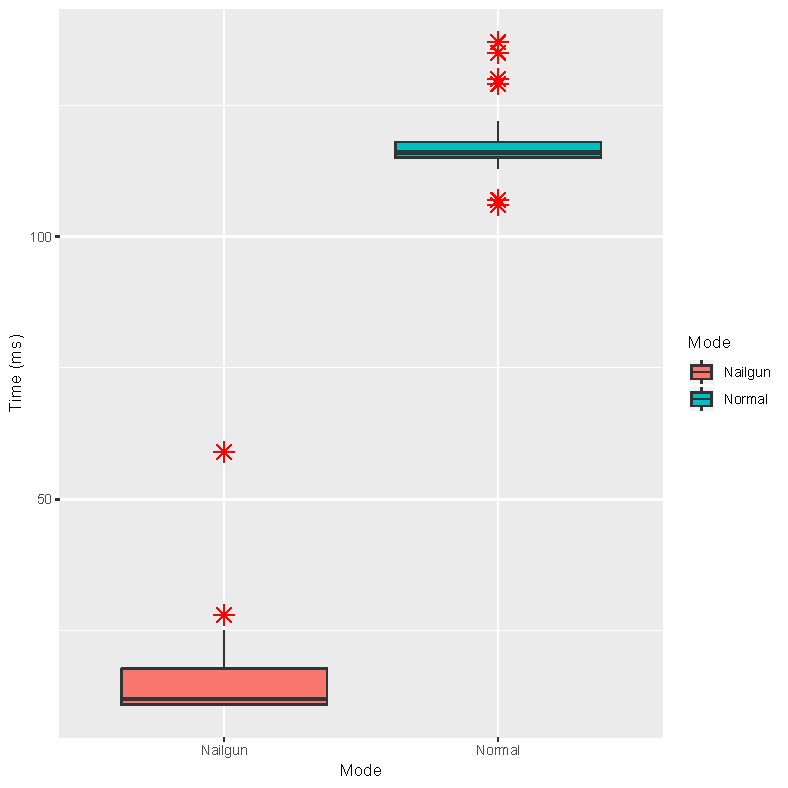
\includegraphics[width=0.45\textwidth]{kuvat/nailgun.pdf}
\par\end{centering}
}\subfloat[Koon optimointi Proguardilla.]{\begin{centering}
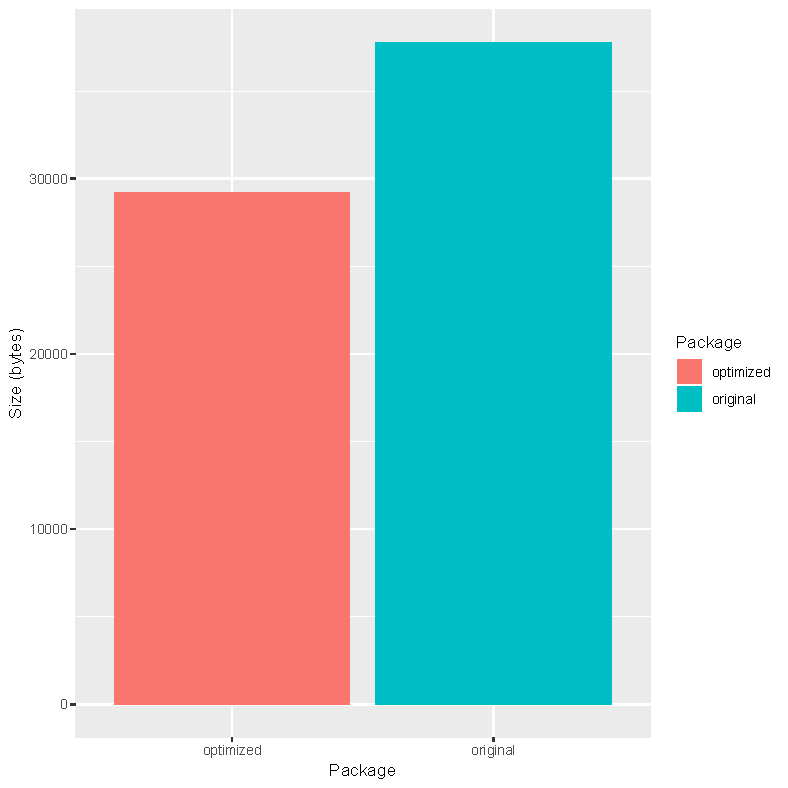
\includegraphics[width=0.45\textwidth]{kuvat/proguard.pdf}
\par\end{centering}
}\caption{Optimointia kahdella eri tavalla.\label{fig:Optimointia-kahdella-eri}}

\end{figure}



%\input{file_name_of_chapter_x}
%\input{file_name_of_chapter_y}

\begin{comment}
The thesis main content ends here.
\end{comment}
\printbibliography

\begin{comment}
Create your appendix chapters with command \textbackslash appchapter\{some
name\} instead of \textbackslash chapter\{some name\} for the automagic
page counting to work!
\end{comment}


\appchapter{Liitedokumentti}

Tässä esimerkki\pagebreak{}

kaksisivuisesta liitteestä.

\appchapter{Liitedokumentti 2}

Tässä esimerkki\pagebreak{}

toisesta kaksisivuisesta liitteestä.

\begin{comment}
main document ends here
\end{comment}

\end{document}
